\subsection{Deep Learning}
I modelli di Deep Learning vengono progettati per analizzare continuamente i dati con una struttura logica simile a quella utilizzata dagli esseri umani per trarre conclusioni. Per raggiungere questo obiettivo, le applicazioni di deep learning si avvalgono di una rete neurale artificiale a più strati, solitamente composte da: un livello di input, uno o più livelli nascosti (\textit{Hidden Layers}) e un livello di output. Ciascun nodo, o neurone artificiale, si connette ad un altro e ha un peso e una soglia associati. Se l'output di qualsiasi singolo nodo è al di sopra del valore di soglia specificato, tale nodo viene attivato, inviando i dati al successivo livello della rete. In caso contrario, non viene passato alcun dato al livello successivo della rete.

I percettroni multistrato vengono addestrati su coppie input-output e imparano a modellare le dipendenze tra ingresso e uscita. L'addestramento comporta la regolazione dei pesi o dei bias ad ogni strato della rete mediante l'utilizzo del backpropagation, un algoritmo di apprendimento supervisionato. La retropropagazione dell'errore cerca il valore minimo della funzione di errore nello spazio dei pesi usando la tecnica del \textit{gradient descent}. I pesi che minimizzano la funzione di errore sono poi considerati una soluzione al problema di apprendimento. 

Una prima caratteristica fondamentale di tali reti è che sono in grado di apprendere, in maniera autonoma e contestuale, le modalità con le quali combinare al meglio le informazioni ricevute per la risoluzione di un compito specifico.

Una seconda caratteristica è che, in maniera similare al cervello umano, sono in grado di imparare dalle loro esperienze, ossia di migliorare le proprie prestazioni nella risoluzione di un problema complesso in funzione della quantità di esempi con cui sono addestrati.
\begin{figure}[hbt!]
    \centering
    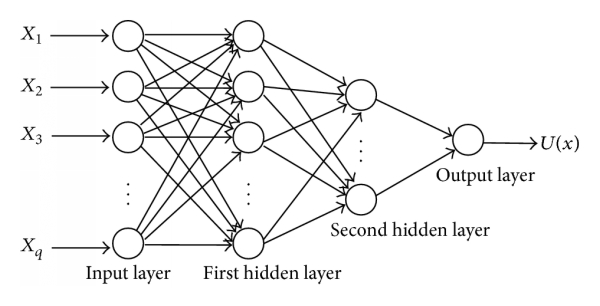
\includegraphics[width=0.8\textwidth]{img/ann.jpg}
    \caption{Esempio di una rete neurale artificiale}
    \label{fig:ann}
\end{figure}
\newpage
Tali reti sono in grado di elaborare, però, come input, solo dati numerici e non stringhe testuali. Questa è una delle motivazioni per le quali le prime applicazioni di successo del deep learning hanno riguardato il trattamento di immagini o segnali. Ad oggi sono state sviluppate diverse tecniche per la mappatura di contenuti testuali in vettori di numeri reali che permettono alle reti neurali di elaborare anche informazioni derivanti da corpus linguistici e pertanto essere impiegate per la risoluzione di task di Natural Language Processing.

Nei capitoli successivi tratteremo il concetto di \textbf{Word Embedding}, l'insieme delle tecniche il cui scopo è proprio quello di eseguire questa mappatura.